\subsection{Dynamics}
We implemented the velocity Verlet algorithm and a Langevin integrator. The velocity Verlet algorithm was used to check the correctness of the potentials and interaction forces by means of energy conservation when not coupled to an external heat bath. All actual simulations were carried out using the Langevin integrator.

The Langevin integrator is a variant of the BBK type integrator due to Br{\"u}nger, Brooks and Karplus \cite{brunger1984stochastic}. Using a velocity Verlet style algorithm, the Langevin equation
\begin{equation}
m a(t) = F(t) - \gamma m v(t) + R(t)
\end{equation}
is discretized and integrated. Here, $\gamma$ is a friction coefficient and $R(t)$ is a gaussian stochastic force with correlation function $\langle\gamma(t), \gamma(t')\rangle = 2 m k_\text{B} T \gamma \delta(t-t')$.

At each iteration, the velocities $v$ first get updated by a half timestep
\begin{equation}
v\left(t + \frac{\Delta t}{2}\right)
= \left(1 - \gamma\frac{\Delta t}{2}\right) v(t)
	+ \frac{\Delta t}{2m} [F(t) + R(t)],
\end{equation}
after which the positions $r$ can be updated to
\begin{equation}
r(t + \Delta t)
= r(t) + v\left(t + \frac{\Delta t}{2}\right) \Delta t.
\end{equation}
With the positions updated, the new forces $F$ can be calculated. With these forces, the velocities can once again be half stepped according to
\begin{equation}
v(t + \Delta t) = \left(1 + \gamma \frac{\Delta t}{2}\right)^{-1}
\left\{
	v\left(t + \frac{\Delta t}{2}\right)
	+ \frac{\Delta t}{2m} \left[
			F(t + \Delta t) + R(t + \Delta t)
	\right]
\right\}.
\end{equation}
The discretized random force $R$ is given by a gaussian random variable with variance $2 m k_\text{B} T \gamma / \Delta t$.

The time step was chosen as large as possible, whilst stil maintaining acceptable errors (as judged, for instance, by examining energy conservation in the Verlet integrator, and stability in the Langevin integrator).
We eventually settled on a timestep of 15\,fs. If there would have been more time, we would have probably opted for a more comfortable timestep of $(5\sim10)$\,fs.

The appropriate friction coefficient was determined by comparing simulated diffusion constants with experimental data. We ended up on a value of $\gamma = 5 \times 10^{12} s^{-1}$, yielding a diffusion coefficient of $(1.3 \pm 0.1) \times 10^{-10}$\,m$^2$/s for a 12 base pair single strand of Adenine at 300\,K and a salt concentration of $[\text{Na}^+] = 50$\,mM.
Figure \ref{diffusion} shows the squared displacements of the simulations that were performed to achieve this result. This is in good agreement with the experimentally determined value of $(1.34 \pm 0.09) \times 10^{-10}$\,m$^2$/s \cite{stellwagen2001measuring, bonifacio1997comparison, eimer1991rotational}. 

\begin{figure}[htb]
       \begin{center}
               \scalebox{0.9}{
                        \nonstopmode
                        % GNUPLOT: LaTeX picture with Postscript
\begingroup
  \makeatletter
  \providecommand\color[2][]{%
    \GenericError{(gnuplot) \space\space\space\@spaces}{%
      Package color not loaded in conjunction with
      terminal option `colourtext'%
    }{See the gnuplot documentation for explanation.%
    }{Either use 'blacktext' in gnuplot or load the package
      color.sty in LaTeX.}%
    \renewcommand\color[2][]{}%
  }%
  \providecommand\includegraphics[2][]{%
    \GenericError{(gnuplot) \space\space\space\@spaces}{%
      Package graphicx or graphics not loaded%
    }{See the gnuplot documentation for explanation.%
    }{The gnuplot epslatex terminal needs graphicx.sty or graphics.sty.}%
    \renewcommand\includegraphics[2][]{}%
  }%
  \providecommand\rotatebox[2]{#2}%
  \@ifundefined{ifGPcolor}{%
    \newif\ifGPcolor
    \GPcolortrue
  }{}%
  \@ifundefined{ifGPblacktext}{%
    \newif\ifGPblacktext
    \GPblacktexttrue
  }{}%
  % define a \g@addto@macro without @ in the name:
  \let\gplgaddtomacro\g@addto@macro
  % define empty templates for all commands taking text:
  \gdef\gplbacktext{}%
  \gdef\gplfronttext{}%
  \makeatother
  \ifGPblacktext
    % no textcolor at all
    \def\colorrgb#1{}%
    \def\colorgray#1{}%
  \else
    % gray or color?
    \ifGPcolor
      \def\colorrgb#1{\color[rgb]{#1}}%
      \def\colorgray#1{\color[gray]{#1}}%
      \expandafter\def\csname LTw\endcsname{\color{white}}%
      \expandafter\def\csname LTb\endcsname{\color{black}}%
      \expandafter\def\csname LTa\endcsname{\color{black}}%
      \expandafter\def\csname LT0\endcsname{\color[rgb]{1,0,0}}%
      \expandafter\def\csname LT1\endcsname{\color[rgb]{0,1,0}}%
      \expandafter\def\csname LT2\endcsname{\color[rgb]{0,0,1}}%
      \expandafter\def\csname LT3\endcsname{\color[rgb]{1,0,1}}%
      \expandafter\def\csname LT4\endcsname{\color[rgb]{0,1,1}}%
      \expandafter\def\csname LT5\endcsname{\color[rgb]{1,1,0}}%
      \expandafter\def\csname LT6\endcsname{\color[rgb]{0,0,0}}%
      \expandafter\def\csname LT7\endcsname{\color[rgb]{1,0.3,0}}%
      \expandafter\def\csname LT8\endcsname{\color[rgb]{0.5,0.5,0.5}}%
    \else
      % gray
      \def\colorrgb#1{\color{black}}%
      \def\colorgray#1{\color[gray]{#1}}%
      \expandafter\def\csname LTw\endcsname{\color{white}}%
      \expandafter\def\csname LTb\endcsname{\color{black}}%
      \expandafter\def\csname LTa\endcsname{\color{black}}%
      \expandafter\def\csname LT0\endcsname{\color{black}}%
      \expandafter\def\csname LT1\endcsname{\color{black}}%
      \expandafter\def\csname LT2\endcsname{\color{black}}%
      \expandafter\def\csname LT3\endcsname{\color{black}}%
      \expandafter\def\csname LT4\endcsname{\color{black}}%
      \expandafter\def\csname LT5\endcsname{\color{black}}%
      \expandafter\def\csname LT6\endcsname{\color{black}}%
      \expandafter\def\csname LT7\endcsname{\color{black}}%
      \expandafter\def\csname LT8\endcsname{\color{black}}%
    \fi
  \fi
  \setlength{\unitlength}{0.0500bp}%
  \begin{picture}(9600.00,7680.00)%
    \gplgaddtomacro\gplbacktext{%
      \colorrgb{0.00,0.00,0.00}%
      \put(1116,845){\makebox(0,0)[r]{\strut{}0}}%
      \colorrgb{0.00,0.00,0.00}%
      \put(1116,2097){\makebox(0,0)[r]{\strut{}0.5}}%
      \colorrgb{0.00,0.00,0.00}%
      \put(1116,3348){\makebox(0,0)[r]{\strut{}1}}%
      \colorrgb{0.00,0.00,0.00}%
      \put(1116,4600){\makebox(0,0)[r]{\strut{}1.5}}%
      \colorrgb{0.00,0.00,0.00}%
      \put(1116,5851){\makebox(0,0)[r]{\strut{}2}}%
      \colorrgb{0.00,0.00,0.00}%
      \put(1116,7103){\makebox(0,0)[r]{\strut{}2.5}}%
      \colorrgb{0.00,0.00,0.00}%
      \put(1248,625){\makebox(0,0){\strut{}0}}%
      \colorrgb{0.00,0.00,0.00}%
      \put(2736,625){\makebox(0,0){\strut{}0.2}}%
      \colorrgb{0.00,0.00,0.00}%
      \put(4224,625){\makebox(0,0){\strut{}0.4}}%
      \colorrgb{0.00,0.00,0.00}%
      \put(5712,625){\makebox(0,0){\strut{}0.6}}%
      \colorrgb{0.00,0.00,0.00}%
      \put(7200,625){\makebox(0,0){\strut{}0.8}}%
      \colorrgb{0.00,0.00,0.00}%
      \put(8688,625){\makebox(0,0){\strut{}1}}%
      \colorrgb{0.00,0.00,0.00}%
      \put(478,3974){\rotatebox{90}{\makebox(0,0){\strut{}\rule{0pt}{-1.5cm}squared displacement ($10^{15}$\,m$^2$)}}}%
      \colorrgb{0.00,0.00,0.00}%
      \put(4968,295){\makebox(0,0){\strut{}time ($\mu$s)}}%
    }%
    \gplgaddtomacro\gplfronttext{%
    }%
    \gplbacktext
    \put(0,0){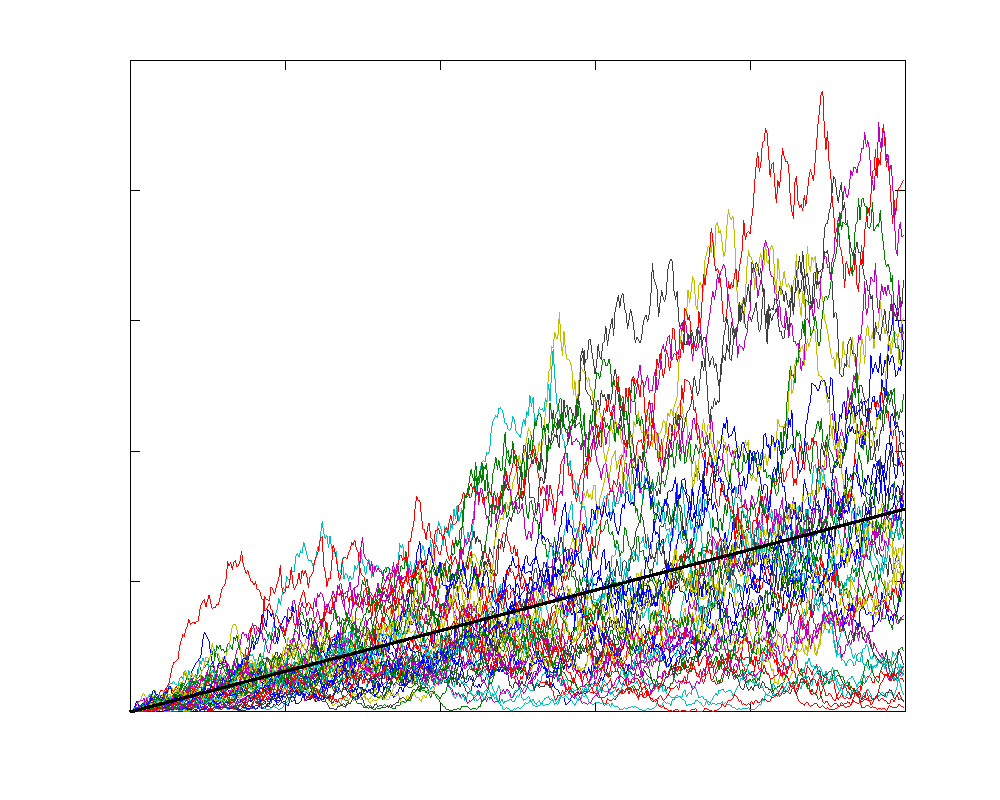
\includegraphics{images/diffusion}}%
    \gplfronttext
  \end{picture}%
\endgroup

                        \errorstopmode
                        \rule[-0.5cm]{0cm}{0cm}}
                \caption{Diffusion of a 12 monomer single strand of Adenine. Shown are the squared displacements of 45 individual simulations at 300\,K and with friction $\gamma = 5 \times 10^{12}$. The black line is the $6Dt$ mean squared displacement curve for the fitted value of $D = (1.3 \pm 0.1) \times 10^{-10}$\,m$^2$/s.}
		\label{diffusion}
        \end{center}
\end{figure}



